\chapter{Probabilistic Modelling}
\label{c:ml-background}

% \note{Machine learning stuff, around 10 pages ..?}

% \section{Probability}
% RANDOM VARIABLES
% ADDING PROBABILITLIES
% JOINT VARIABLES, CONDITIONING
 %FACTORISATION AND INDEPDENCE
 %GRAPHICAL MODEL
% BAYES RULES
% MARGINISALISATION
% COMMON DISTRIBUTIONS: DIRICHLET, MULTINOMIAL, GAUSSIAN

\section{Bayesian Inference}

At the heart of this thesis is the grouping and generative modelling of peaks that are structurally or chemically related in some manner. As no ground truth is available for use as the training data, the problem of finding these groups of related peaks are often approached as an unsupervised learning problem. In the unsupervised learning approach, broadly speaking our task is to separate peaks into \emph{clusters}, where members of the cluster are related through sharing some commonalities, e.g. from being the ionisation products of the same compound or from being members of the same chemical substructure shared by many metabolites.

One way to perform clustering is to try and model the generative process that produces the observed data. In this manner, peak features explained by the same underlying latent variables are considered to be in the same cluster. For example, the chromatographic process separates metabolites by their chemical properties. Peaks that are related through being the ionisation products of the same metabolite will co-elute and have similar chromatographic profiles. A group of peak features that have similar retention time (RT) values can be therefore be modelled as being generated by the same metabolite. 

A principled way to model a generative process is through Bayesian inference. Let $\mathbf{Y}=y_1,y_2,...,y_n$ be the set of $N$ observed data and $\theta$ the parameter of interest to the generative process that produces $\mathbf{y}$. In Bayesian inference, we begin by specifying a \emph{prior} distribution over $\theta$. Through the application of Bayes rule, this prior distribution is updated by the \emph{likelihood} of seeing the observed data given our hypothesis on $\theta$. This results in a \emph{posterior} distribution:
\begin{equation}
p(\theta \vert \mathbf{y})=\frac{p(\mathbf{y},\theta)}{p(\mathbf{y})}=\frac{p(\mathbf{y} \vert \theta)p(\theta)}{p(\mathbf{y})}=\frac{p(\mathbf{y} \vert \theta)p(\theta)}{\int_{\theta} p(\mathbf{y} \vert \theta)p(\theta) \enspace d\theta}
\label{eq:background-bayesian}
\end{equation}
In eq. (\ref{eq:background-bayesian}), $p(\mathbf{y},\theta)$ is the joint distribution between the data $\mathbf{y}$ and the model parameter $\theta$. This can be factorised into a product of $p(\mathbf{y} \vert \theta)$, which is the likelihood of observing the data $\mathbf{y}$ given the model parameter $\theta$, and $p(\theta)$, which is the prior distribution on the model parameter $\theta$. Normalising the joint distribution by the \emph{marginal likelihood} or evidence $p(\mathbf{y})$ produces the posterior distribution $p(\theta \vert \mathbf{y})$, which is the probability of model parameter $\theta$ given the data. Inferring model parameters given the observed data is usually what we are interested in.

Using the posterior distribution, we can make a prediction on a new feature, $y_{new}$ by averaging over all values of $\theta$. This results in the posterior predictive distribution:
\begin{equation}
p(y_{new} \vert \mathbf{y})=\int_{\theta} p(y_{new} \vert \theta) p(\theta \vert \mathbf{y}) \enspace d\theta
\label{eq:background-posterior-predictive}
\end{equation}
% It is also possible to sequentially update the posterior distribution $p(\theta \vert \mathbf{y})$ given $y_{new}$. This makes Bayesian inference suitable for online learning.
% \begin{equation}
% p(\theta \vert \mathbf{y},y_{new})=\frac{p(y_{new}  \vert \theta)p(\theta \vert \mathbf{y})}{\int_{\theta} p(y_{new}  \vert \theta)p(\theta \vert \mathbf{y}) d\theta}
% \end{equation}
In many cases, the integral in eqs. (\ref{eq:background-bayesian}) and (\ref{eq:background-posterior-predictive}) cannot be solved analytically and have to be approximated through maximum likelihood or sampling-based approaches.

\subsection{Example: Modelling Coin Tosses}
\label{sub:background-coin-toss}

We illustrate the principle of Bayesian inference using an illustrative coin toss experiment. This will be a very brief example, and interested readers are referred to textbooks such as \cite{rogers2015first, gelman2014bayesian, murphy2012machine} for more details. 

Suppose we have a coin and we are interested in knowing $P(head)$, the probability of seeing a head in a coin toss experiment. We use 1 to encode a head outcome and 0 to encode a tail outcome. Let $y_n$ be a random variable that stores the outcome (0 or 1) of any $n$-th coin toss, The probability of seeing a head in the $n$-th coin toss is $P(y_n=1)=\theta$, while the probability of seeing a tail is $P(y_n=0)=1-\theta$. From this series of Bernoulli trials, we obtain $\mathbf{y}=y_1,y_2,...,y_n$, the set of observations of all the coin toss outcomes. After performing $N$ coin tosses, let $a$ be the total number of heads while $b$ the total number of tails. Assuming that each coin toss is independent of the others, the likelihood of the entire observations is: 
\begin{equation}
p(\mathbf{y} \vert \theta)=\theta^a(1-\theta)^b
\label{eq:example-likelihood}
\end{equation}
Here, $\theta$ serves as the parameter of the likelihood in our model that we would like to infer. Following the Bayesian approach, we also require a prior distribution that specifies our belief on the values $\theta$ may take. As $\theta$ ranges from 0 to 1, we need a prior distribution with a support over the interval $[0, 1]$. For mathematical convenience, a prior distribution that has the same form as the likelihood (a \emph{conjugate prior}) can be chosen. In this case, the beta distribution is a suitable conjugate prior distribution to the likelihood in eq. (\ref{eq:example-likelihood}). The beta distribution itself has two shape parameters $\alpha$ and $\beta$ and takes the form of:
\begin{equation}
p(\theta \vert \alpha,\beta)=\frac{\theta^{(\alpha-1)}(1-\theta)^{(\beta-1)}}{B(\alpha,\beta)}
\end{equation}
where $B(\alpha,\beta)=\frac{\Gamma(\alpha)\Gamma(\beta)}{\Gamma(\alpha+\beta)}$ is the normalisation constant to make the total probability integrates to 1. Ignoring this constant, we arrive at a proportional form for the prior that is the same as the likelihood:
\begin{equation}
p(\theta \vert \alpha,\beta) \propto \theta^{(\alpha-1)}(1-\theta)^{(\beta-1)}
\label{eq:example-beta-parameters}
\end{equation}
In eq. (\ref{eq:example-beta-parameters}), $\alpha$ and $\beta$ are the \emph{hyperparameters} of the prior distribution. They can be set to encode our prior beliefs on the values for $\theta$. For instance, if we have no assumption about the coin at all, we may believe that all values for $\theta$ is equally likely. Setting $\alpha$ and $\beta$ to 1 will result in a uniform distribution that does not favour any value of $\theta$ (Figure~\ref{fig:beta-prior}A). If we think that we have a fair coin on our hand, setting $\alpha$ and $\beta$ to 10 results in a distribution that is concentrated around 0.5 (Figure~\ref{fig:beta-prior}B). If we think that we have a biased coin, setting $\alpha$ to 10 and $\beta$ to 1 results in a biased distribution for $\theta$ that favours heads (Figure~\ref{fig:beta-prior}C). In this manner, the hyperparameters allow us to encode our prior belief in the model. 
\begin{figure}
\noindent \begin{centering}
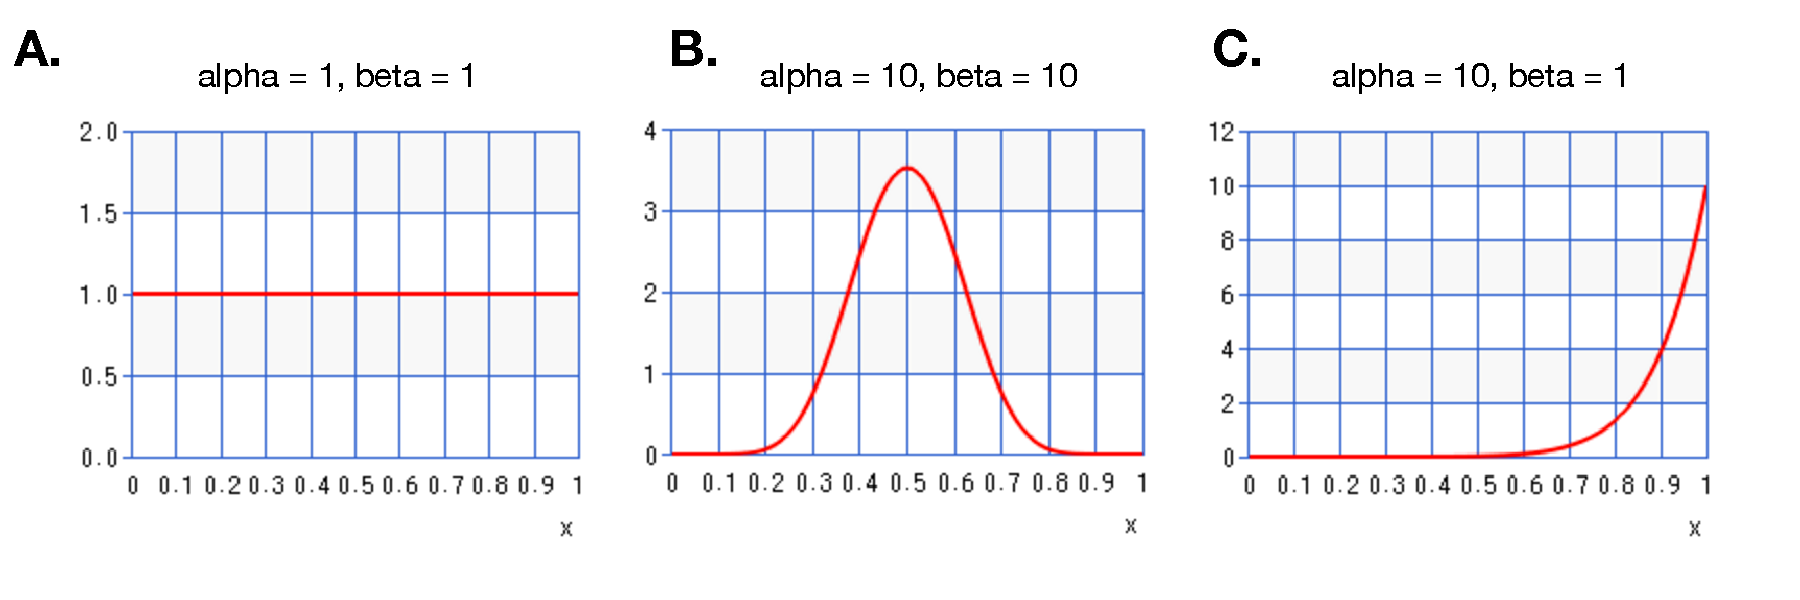
\includegraphics[width=1.0\textwidth]{03-machine-learning/figures/beta_prior.pdf}
\par\end{centering}
\caption{\label{fig:beta-prior}Different prior beliefs on $\theta$ from changing the hyperparameters: \textbf{(A.)} No assumption about the coin, \textbf{(B.)} we have a fair coin, and \textbf{(C.)} we have a biased coin.}
\end{figure}

To obtain the unnormalised posterior distribution, we multiply the likelihood and the prior, resulting in
\begin{equation}
\begin{aligned}
p(\theta \vert \mathbf{y}) \propto p(\mathbf{y} \vert \theta)p(\theta) &= \bigg[\theta^a (1-\theta)^b\bigg] \bigg[\theta^{(\alpha-1)} (1-\theta)^{(\beta-1)}\bigg] \\
                                                                               &= \theta^{(a+\alpha-1)} (1-\theta)^{(b+\beta-1)} \\
\label{eq:background-posterior}
\end{aligned}
\end{equation}
We see from eq. (\ref{eq:background-posterior}) that the unnormalised posterior distribution is proportional to another beta distribution parameterised by the scale parameters $a+\alpha$ and $b+\beta$. We can normalise this by $B(a+\alpha,b+\beta)$ to make it a probability distribution that integrates to 1. To use the posterior distribution for predicting that the probability for the next coin toss $y_{new}$ is a head, we compute the posterior predictive distribution:
\begin{equation}
\begin{aligned}
p(y_{new}=1 \vert \mathbf{y}) &= \int_{\theta} p(y_{new}=1 \vert \theta) \enspace p(\theta \vert \mathbf{y}) \enspace d\theta \\
                                 &= \int_{\theta} \theta \enspace p(\theta \vert \mathbf{y}) \enspace d\theta \\
                                 &= \mathbf{E}(\theta \vert \mathbf{y})
\end{aligned}
\label{eq:example-posterior-predictive}
\end{equation}
where $\mathbf{E}(\theta)$ is the expected value of $\theta$ conditioned on $\mathbf{y}$. The expected value (mean) of a general beta distribution parameterised by $a$ and $b$ is $\frac{a}{a+b}$. Since $p(\theta \vert \mathbf{y})$ is a beta distribution parameterised by $a+\alpha$ and $b+\beta$, $\mathbf{E}(\theta \vert X)$ is therefore $\frac{a+\alpha}{a+b+\alpha+\beta}$. 

While simple, this example serves to illustrate the principle of Bayesian inference. We start with an initial hypothesis on the values $\theta$ may take. This is encoded in the hyperparameters of the prior distribution on $\theta$. Observations are used to update this distribution, resulting in a posterior distribution. Inference on model parameters can then be made using this posterior distribution. The same principle will be applied in the following section that uses a mixture model to generatively model peak data.

\section{Mixture Model Clustering}

We now introduce a more complex model to capture the dependencies of peak features in our LC-MS data. Recall that peak features that are related in some manner can be explained (generated) by the same cluster. Statistical \emph{mixture model} represents each cluster by a probability distribution. A cluster is represented as a component in the mixture model. The choice of which probability distribution is used as the component is usually determined by the type of observed data. For instance, the Gaussian distribution can be used as the mixture component where the data is continuous, while the multinomial distribution is used for discrete count data. We then pick one of the clustering with a certain probability, and generate a data point by sampling from the cluster-specific probability distribution. Mixture models are the building blocks of more complex probabilistic models where it is assumed that the observed data can be explained by the presence of some unknown latent variables. Particularly for LC-MS data, mixture models have been used as the generative models to cluster peaks in \cite{Rogers2012,Daly2014}.

To illustrate with an example, here we outline the construction of a mixture model to cluster peaks in a single LC-MS run by their retention time (RT) values. The Gaussian mixture model described here follows from \cite{Rasmussen2000}: it starts from having a finite number of components and will subsequently be extended to an infinite mixture model where the number of components is unbounded. As a generative process, we assume a compound (metabolite/peptide) generates a set of peaks that share close RT values as they co-elute from the column. Peaks that are related to the same compound can therefore be clustered according to their RT values. Our LC-MS run is represented as $\mathbf{y}=\{y_{1},y_{2},...,y_{n}\}$ where each $y_n$ is the RT value of a peak. The mixture model is a weighted sum of its $K$ components, where each component corresponding to a cluster, is represented by a probability distribution. Because each data point is a scalar, we use a univariate Gaussian distribution as the mixture component. Each mixture component has an unknown mean $\mu_{k}$ but a known variance $\sigma^2$. The choice of using a known and fixed variance for all components in the model is motivated by the following assumptions: \textbf{(1)} the retention time drift of observed peaks is broadly similar across the compounds being measured, and \textbf{(2)} this parameter can be set by the user based on his knowledge on the characteristic RT drifts of the LC instrument. For a single peak, its mixture model likelihood is given by:
\begin{equation}
p(y_n \vert \boldsymbol{\mu},\boldsymbol{\pi}) = \sum_{k=1}^{K} \pi_k \mathcal{N}(y_n \vert \mu_k,\sigma^2)
\end{equation}
where $\pi_k$ and $\mu_k$ are the mixture proportion and mean of the $k$-th component. The mixture proportion tells us how much of the density is contributed by a mixture component. In this manner, $\pi_{k}>0$ and $\sum_{k=1}^{K}\pi_{k}=1$. $\boldsymbol{\mu}=\{\mu_{1},...,\mu_{k}\}$ is the vector over all component means, while $\boldsymbol{\pi}=\{\pi_{1},...,\pi_{k}\}$ is the vector over all mixture proportions.

We assume that each peak is generated by exactly one mixture component (cluster) and introduce a random variable $z_{nk}$ to store the assignment of peak $n$ to cluster $k$. In this manner, $z_{nk}=1$ if peak $n$ is assigned to cluster $k$, and 0 otherwise. Each peak can only be assigned to one cluster ($\sum_{k} z_{nk} = 1$). For a peak, we can store its cluster assignments in a vector $\boldsymbol{z}_{n}$. Let $\boldsymbol{Z}$ is the set of all indicator vectors for all peaks. Collectively for all peaks, the joint likelihood of the observed data and the cluster assignments is:
\begin{equation}
p(\boldsymbol{y},\boldsymbol{Z}  \vert \boldsymbol{\mu},\boldsymbol{\pi}) = \prod_{n=1}^{N} \prod_{k=1}^{K} \big[ \pi_k \enspace \mathcal{N}(y_n \vert \mu_k,\sigma^2) \big]^{\boldsymbol{z}_{nk}}
\label{eq:background-mixture-likelihood}
\end{equation}
For each peak, its cluster assignment vector,  $\boldsymbol{z}_n$, can be modelled by a multinomial distribution having the parameter vector $\boldsymbol{\pi}$. For all peaks, this results in:
\begin{equation}
\begin{aligned}
p(\boldsymbol{Z} \vert \boldsymbol{\pi}) &\propto \prod_{n=1}^N \prod_{k=1}^{K} \pi_k^{z_{nk}} \\
                                                              &= \prod_{k=1}^{K} \pi_k^{c_{k}}
\end{aligned}
\label{eq:background-z-given-pi}
\end{equation}
where $c_{k} = \sum_n z_{nk}$ is the count of peaks assigned to the $k$-th cluster. We also place a prior distribution on $\boldsymbol{\pi}$. Due to its conjugacy, we use a Dirichlet distribution parameterised by the parameter vector $\boldsymbol{\alpha}=[\alpha_1,\alpha_2,...,\alpha_k]^T$ as the prior. This results in:
\begin{equation}
\begin{aligned}
p(\boldsymbol{\pi} \vert \boldsymbol{\alpha}) &= \frac{\Gamma(\sum_{k} \alpha_{k})}{\prod_{k} \Gamma(\alpha_k)}  \prod_{k=1}^{K} \pi_k^{\alpha_{k}-1} \\
                                                                      &\propto \prod_{k=1}^{K} \pi_k^{\alpha_{k}-1}
\end{aligned}
\label{eq:background-pi-given-alpha}
\end{equation}
We also need to define the prior distribution for the $\mu_k$s. We assume this comes from another Gaussian distribution having the mean $\mu_0$ and the variance $\sigma^2_0$ given the hyperparameters. Assuming that the means for each cluster are independent from each other given the hyperparameters, we obtain:
\begin{equation}
p(\boldsymbol{\mu} \vert \mu_0, \sigma^2_0) = \prod_{k=1}^K \mathcal{N}(\mu_k \vert \mu_0, \sigma^2_0)
\label{eq:background-prior-gaussian}
\end{equation}

The joint probability distribution of the model parameters and data is given by $p(\boldsymbol{y}, \boldsymbol{Z}, \boldsymbol{\mu}, \boldsymbol{\pi} \vert \boldsymbol{\alpha}, \allowbreak \mu_0,\sigma_0^2)$, which using eqs. (\ref{eq:background-mixture-likelihood}-\ref{eq:background-prior-gaussian}), can be factorised into eq. (\ref{eq:example-full-joint-dist}). 
\begin{equation}
p(\boldsymbol{y}, \boldsymbol{Z}, \boldsymbol{\mu}, \boldsymbol{\pi} \vert \boldsymbol{\alpha},\mu_0,\sigma_0^2) = p(\boldsymbol{y} \vert \boldsymbol{Z}, \boldsymbol{\mu},\boldsymbol{\pi}) p(\boldsymbol{Z} \vert \boldsymbol{\pi}) p(\boldsymbol{\pi} \vert \boldsymbol{\alpha}) p(\boldsymbol{\mu} \vert \mu_0, \sigma_0^2)
\label{eq:example-full-joint-dist}
\end{equation}

This factorisation of the joint distribution can also be illustrated as a graphical model (Figure~\ref{fig:background-mixture-plate-diagram}A), which shows the conditional dependencies of random variables in the model. We can also write out the generative process for this finite mixture model as:
\begin{equation}
\begin{aligned}
\boldsymbol{\pi} \vert \boldsymbol{\alpha} &\sim Dir(\boldsymbol{\alpha}) \\
z_{nk}=1 \vert \pi_k                                  &\sim \boldsymbol{\pi} \\
\mu_k \vert \mu_0                                    &\sim \mathcal{N}(\mu_k \vert \mu_0, \sigma_0^2) \\
y_n \vert z_{nk}=1, \mu_k                         &\sim \mathcal{N}(y_n \vert \mu, \sigma^2)
\end{aligned}
\label{eq:background-finite-mixture}
\end{equation}

\begin{figure}[tbh!]
\noindent \begin{centering}
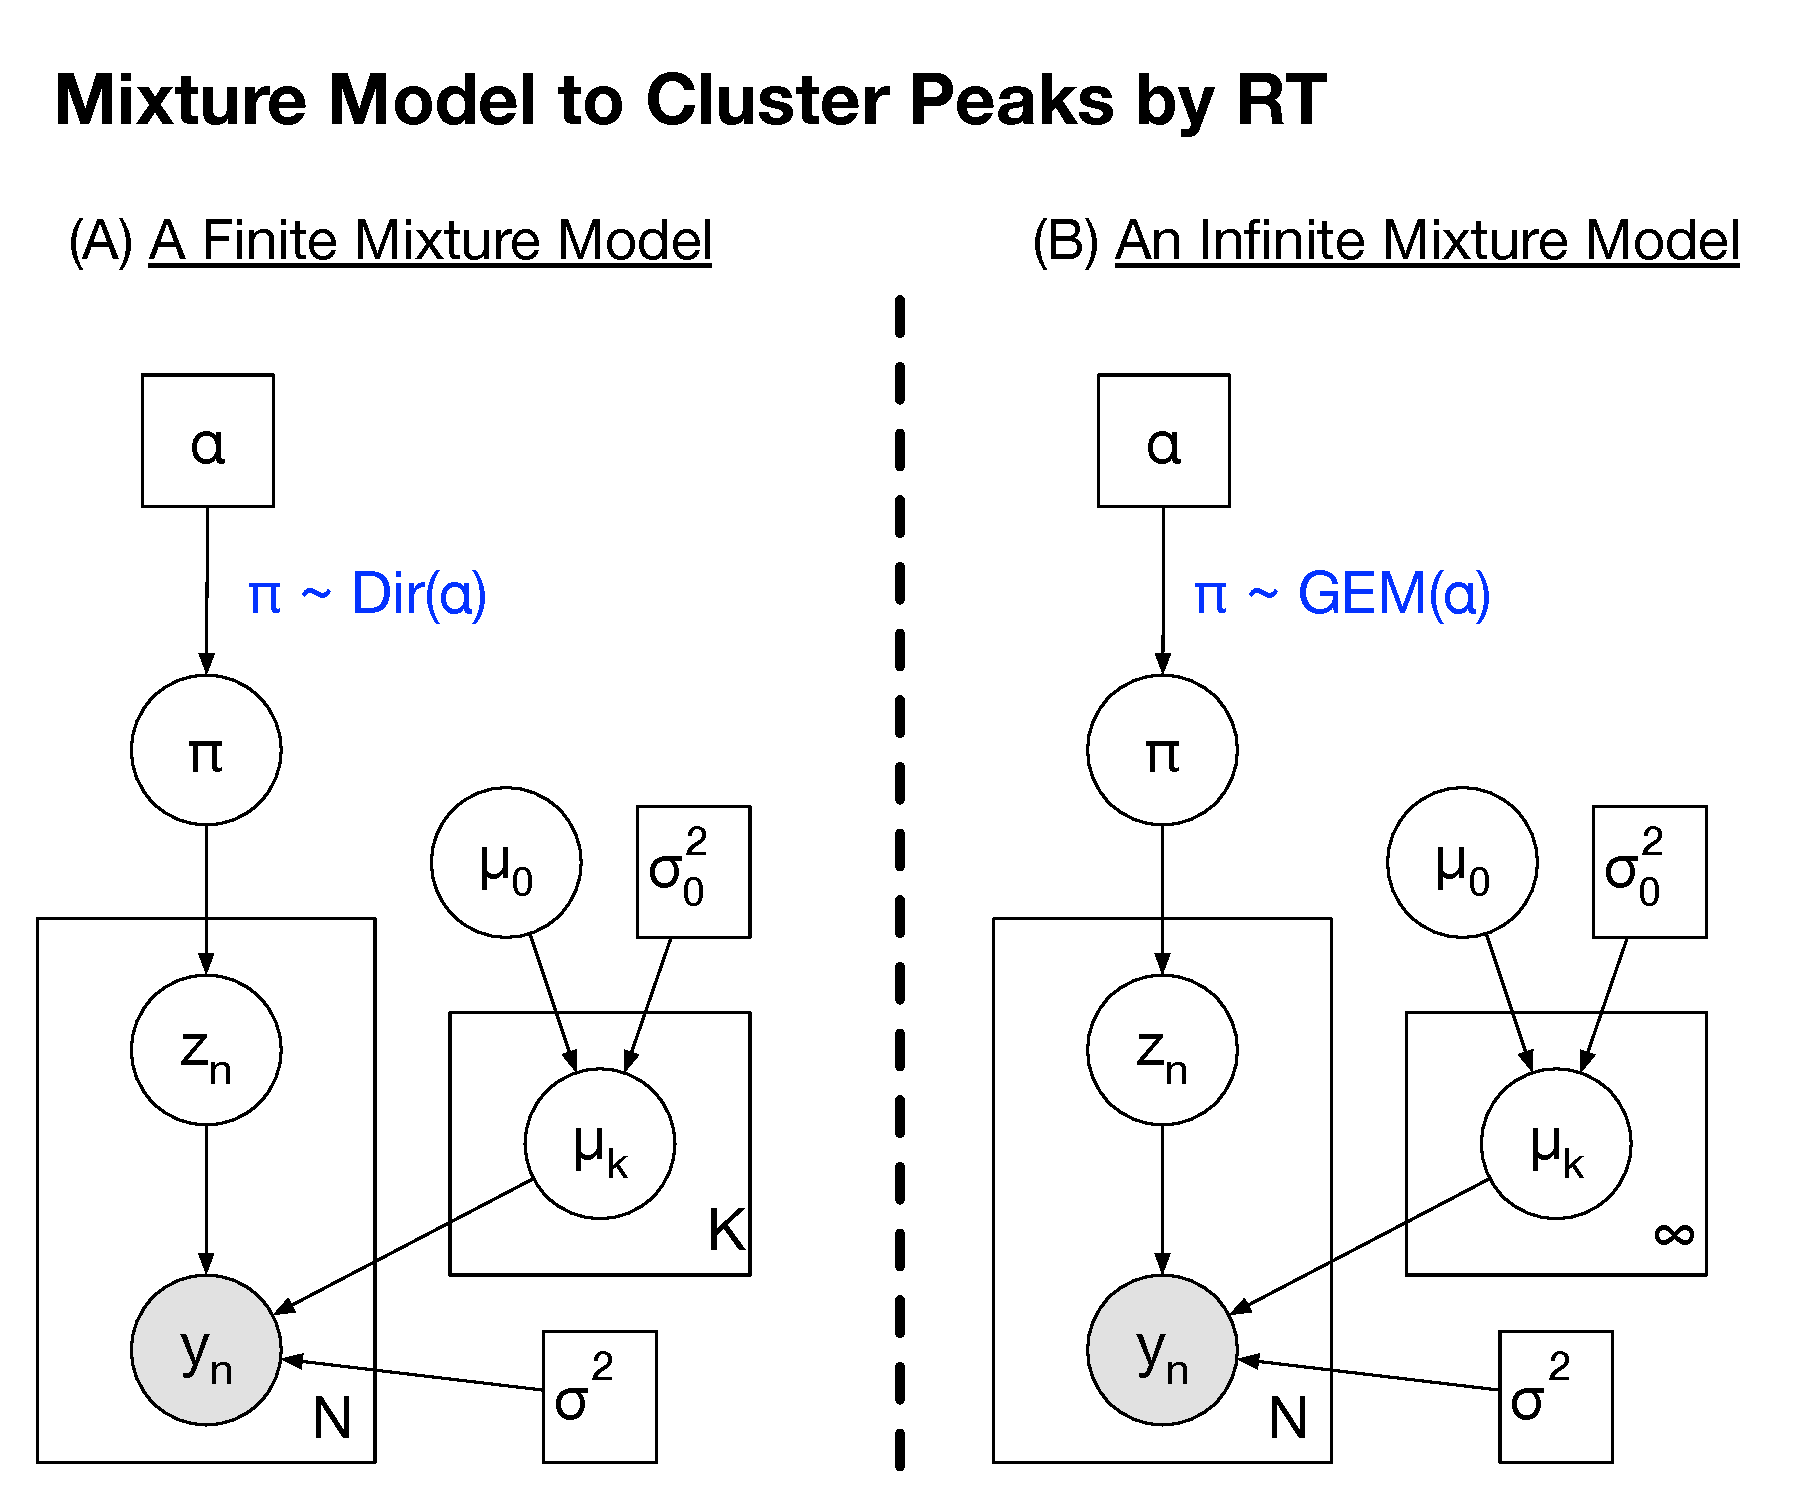
\includegraphics[width=0.8\textwidth]{03-machine-learning/figures/mixture_model.pdf}
\par\end{centering}
\caption{\label{fig:background-mixture-plate-diagram}Graphical models of (1) a finite mixture model, which is extended into (2) an infinite mixture model, to cluster peaks by their retention time (RT) values. Circles denotes random variables, squares denote fixed parameters, while the shaded node denotes an observed peak's RT.}
\end{figure}

\subsection{Gibbs Sampling for an Finite Mixture Model}

Given the joint distribution in eq. (\ref{eq:example-full-joint-dist}), we are interested to infer the posterior distribution on the assignments $\boldsymbol{Z}$, the mixture proportions $\boldsymbol{\pi}$ and the cluster means $\boldsymbol{\mu}$. This is given by:
\begin{equation}
p(\boldsymbol{Z},\boldsymbol{\pi},\boldsymbol{\mu} \vert \boldsymbol{y}, \boldsymbol{\alpha},\mu_0,\sigma_0^2) = \frac{p(\boldsymbol{y}, \boldsymbol{Z}, \boldsymbol{\mu},\boldsymbol{\pi} \vert \boldsymbol{\alpha},\mu_0,\sigma_0^2)}{p(\boldsymbol{y} \vert \alpha,\mu_0,\sigma_0^2)}
\label{eq:background-mixture-posterior}
\end{equation}
Substituting eq. (\ref{eq:example-full-joint-dist}) into the numerator of eq. (\ref{eq:background-mixture-posterior}) results in the following posterior distribution over the parameters that we want to infer:
\begin{equation}
p(\boldsymbol{Z},\boldsymbol{\pi},\boldsymbol{\mu} \vert \boldsymbol{y},\alpha,\mu_0,s_0) \propto p(\boldsymbol{y} \vert \boldsymbol{Z}, \boldsymbol{\mu},\boldsymbol{\pi}) p(\boldsymbol{Z} \vert \boldsymbol{\pi}) p(\boldsymbol{\pi} \vert \boldsymbol{\alpha}) p(\boldsymbol{\mu} \vert \mu_0, s_0)
\label{eq:background-mixture-expanded-posterior}
\end{equation}

In many cases for the more interesting and complex models, the posterior distribution (such as the one in eq. \ref{eq:background-mixture-expanded-posterior}) and also the posterior predictive distribution cannot be derived analytically. Various methods exist to perform posterior inference in a mixture model [REF????], but throughout this thesis, we will use Gibbs sampling, an instance of Markov chain Monte Carlo (MCMC) methods. Gibbs sampling approximates the target posterior distribution by sequentially updating each random variable conditioned on all other random variables in the model. This requires deriving the \emph{conditional distribution} of each random variable that we want to infer. In some cases, obtaining these conditional distributions can be challenging, although the process can be simplified by the independence assumptions of our model (e.g. in assuming that the cluster means are independent) and through the use of the appropriate conjugate prior distributions.  Here we describe the steps required to construct a Gibbs sampler for the mixture model defined in eq. (\ref{eq:background-finite-mixture}).

As the initial step in our Gibbs sampler, we initialise the cluster means $\mu_1,\mu_2,..,\mu_k$ and the mixture proportion $\boldsymbol{\pi}$ by sampling from their respective prior distributions. Then we sequentially sample for new values of $\boldsymbol{Z}$, $\boldsymbol{\mu}$ and $\boldsymbol{\pi}$ from the conditional distributions listed below. 

\begin{enumerate}

\item We can update $\boldsymbol{z}_n$, the membership vector for peak $n$, by updating each of its $k$-th individual entry, i.e. $z_{nk}$. Simplifying eq. (\ref{eq:background-mixture-likelihood}) to consider just one $n$-th peak, we obtain the following after normalisation:
\begin{equation}
P(z_{nk}=1 \vert \boldsymbol{\pi}, y_n, \mu_k) = \frac{\pi_k \enspace \mathcal{N}(y_n \vert \mu_k, \sigma^2)}{\sum_{k=1}^K \pi_k \enspace \mathcal{N}(y_n \vert \mu_k, \sigma_2)}
\label{eq:background-mixture-conditional-z}
\end{equation}

\item As the next step, we also need to update each $\mu_k$ conditioned on the membership vectors $\boldsymbol{Z}$ and the hyperparameters $\mu_0$ and $\sigma_0$. Consider one $k$-th cluster, and let $\boldsymbol{x}={x_1,x_2,...,x_M}$ be the set of peaks currently assigned to that cluster. There are $M$ such peaks, and their joint likelihood is $p(\boldsymbol{x} \vert \mu_k)$. As defined in eq. (\ref{eq:background-prior-gaussian}), we assume that each $\mu_k$ is independent given its conjugate prior $\mathcal{N}(\mu_0, \sigma_0^2)$ . The posterior distribution on $p(\mu_k \vert \boldsymbol{x}, \mu_0)$ is therefore:
\begin{equation}
\begin{aligned}
p(\mu_k \vert \boldsymbol{x}, \mu_0) &\propto p(\boldsymbol{x} \vert \mu_k) \cdot p(\mu_k \vert \mu_0) \\
                                                           &= \prod_{m=1}^{M} \mathcal{N}(x_m \vert \mu_k, \sigma^2) \cdot \mathcal{N}(\mu_k \vert \mu_0, \sigma_0) \\
                                                           &= \prod_{m=1}^{M} \frac{1}{\sqrt{2\sigma^2\pi}} exp\bigg(\frac{-(x_n-\mu_k)^2}{2\sigma^2} \bigg) \cdot \frac{1}{\sqrt{2\sigma_0^2\pi}} exp\bigg(\frac{-(\mu_k-\mu_0)^2}{2\sigma_0^2} \bigg)
\end{aligned}                                                           
\label{eq:background-posterior_mu_k}
\end{equation}
Since $p(\mu_k \vert \boldsymbol{x}, \mu_0)$ is a product of Gaussians, the posterior is proportional to another Gaussian, parameterised by say $\mathcal{N}(\tilde{\mu}, \tilde{\sigma}^2)$. Equating this with eq. (\ref{eq:background-posterior_mu_k}) results in:
\begin{equation}
exp\bigg(\frac{-(\mu_k-\tilde{\mu})^2}{2\tilde{\sigma}^2} \bigg) \propto exp\bigg(\frac{-\sum_{m=1}^{M} (x_m-\mu_k)^2}{2\sigma^2} + \frac{-(\mu_k-\mu_0)^2}{2\sigma_0^2}\bigg)
\label{eq:background-solving-posterior-mu_k}
\end{equation}
Simplifying eq. (\ref{eq:background-solving-posterior-mu_k}) and completing the squares, we obtain the following parameters for $\mathcal{N}(\mu_k \vert \tilde{\mu}, \tilde{\sigma}^2)$:
\begin{equation}
\tilde{\mu} = \tilde{\sigma}^2 \bigg( \frac{\sum_{m=1}^{M} x_m}{\sigma^2} + \frac{\mu_0}{\sigma_0^2} \bigg), \enspace
\tilde{\sigma} = \frac{1}{\frac{M}{\sigma^2} + \frac{1}{\sigma^2_0}} 
\label{eq:background-tilde-mu-sigma}
\end{equation}

\item Finally we also need to update the mixture proportion $\boldsymbol{\pi}$. Putting together the multinomial likelihood and Dirichlet prior in eqs. (\ref{eq:background-z-given-pi}) and (\ref{eq:background-pi-given-alpha}), we obtain a conditional distribution for $\boldsymbol{\pi}$ that is another Dirichlet distribution, parameterised by $[\alpha_{1}+c_{1}, \alpha_{2}+c_{2}, ..., \alpha_{k}+c_{k}]^T$. Each entry in this parameter vector is influenced by two values: the pseudo-count contribution from $\alpha_k$ and the actual counts of peaks currently assigned to cluster $k$ from $c_k$. 
\begin{equation}
\begin{aligned}
p(\boldsymbol{\pi} \vert \boldsymbol{\alpha}, \boldsymbol{Z}) = p(\boldsymbol{Z} \vert \boldsymbol{\pi}) \cdot p(\boldsymbol{\pi} \vert \boldsymbol{\alpha})
                                                                                                &\propto \prod_{k=1}^{K} \pi_k^{\alpha_{k}-1} \cdot \prod_{k=1}^{K} \pi_k^{c_{k}}  \\
                                                                                                &= \prod_{k=1}^{K} \pi_k^{\alpha_{k}+c_{k}-1} \\
                                                                                                &= Dir(\alpha_{1}+c_{1}, \alpha_{2}+c_{2}, ..., \alpha_{k}+c_{k})
\end{aligned}
\label{eq:background-mixture-conditional-pi}
\end{equation}

\end{enumerate}

In Gibbs sampling, each newly updated value is immediately used before sampling for the next value. This sampling of each random variable is repeated until convergence. Often a certain number of initial samples are discarded during the \emph{burn-in} period. Since successive samples are correlated, a certain \emph{thinning} interval is also used to reduce the number of samples used. The resulting samples can now be used to approximate the true posterior distribution of the model. Frequently, the marginal distribution of the random variable of interest is studied. Particularly for our case, often we are interested in the probability of any pair of peaks (or even a set of peaks) to be placed in the same component since, as the subsequent chapters will show, this has a direct application to the problem of peak alignment.

\subsection{Collapsed Gibbs Sampling for an Finite Mixture Model}

As we have chosen conjugate prior distributions on the mixture proportion $\boldsymbol{\pi}$ and also the cluster mean $\mu_k$, it is possible for us to integrate (\emph{collapse}) $\boldsymbol{\pi}$ and $\mu_k$ from the model during Gibbs sampling. This results in a collapsed Gibbs sampler (CGS) where we need not sample $\boldsymbol{\pi}$ and $\mu_k$ explicitly. Collapsing has also been shown to lead to a better model convergence \cite{gelman2014bayesian}. It will also help in the next section when we want to extend our finite mixture model (where the number of components, $K$ is specified) to an infinite mixture model (where the number of components are unbounded) as we do not need to explicitly sample an infinite-dimensional vector $\boldsymbol{\pi}$. 

Specifically in this CGS implementation, we aim to marginalise $\boldsymbol{\pi}$ and $\mu_k$ by integrating them out from the conditional probability for $z_{nk}$, the assignment of peak $n$ to cluster $k$. Collapsing $\boldsymbol{\pi}$ introduces dependencies among all the $\boldsymbol{z}_n$ random variables, so we introduce another notation $\boldsymbol{Z}^{-}$ to mean all other $\boldsymbol{z}_n$s except the one for the current $n$-th peak being sampled upon. Similarly, $\boldsymbol{y}^{-}$ denotes the RT values for other peaks apart from $y_n$. The conditional distribution for $z_{nk}$ in the CGS is given by:
\begin{equation}
\begin{aligned}
p(z_{nk}=1, \boldsymbol{\pi} \vert \boldsymbol{Z}^{-}, \boldsymbol{y}^-, \mu_0, \boldsymbol{\alpha}) \propto p(y_n \vert \boldsymbol{Z}^{-},  \boldsymbol{y}^{-}, \mu_0) \cdot P(z_{nk}=1 \vert \boldsymbol{Z}^{-}, \boldsymbol{\alpha})
\end{aligned}
\label{eq:background-collapsed-gibbs}
\end{equation}
We consider both terms of eq. (\ref{eq:background-collapsed-gibbs}) separately. 
\begin{enumerate}

\item The first term on the right hand side of eq. (\ref{eq:background-collapsed-gibbs}) is the likelihood of $y_n$ to be assigned to cluster $k$. Here, we no longer need to sample for $\mu_k$ as we are integrating over all values of $\mu_k$ using the posterior distribution $\mathcal{N}(\mu_k \vert \tilde{\mu}, \tilde{\sigma}^2)$ defined in eq. (\ref{eq:background-solving-posterior-mu_k}). Instead we can directly compute this likelihood by:
\begin{equation}
\begin{aligned}
p(y_n \vert \boldsymbol{Z}^{-},  \boldsymbol{y}^{-}, \mu_0) &\propto \int p(y_n \vert \mu_k) \cdot p(\mu_k \vert \boldsymbol{Z}^{-},  \boldsymbol{y}^{-}, \mu_0) \enspace d\mu_k \\
                                                                                            &\propto \int \mathcal{N}(y_n \vert \mu_k, \sigma^2) \cdot \mathcal{N}(\mu_k \vert \tilde{\mu}, \tilde{\sigma}^2) \enspace d\mu_k \\
                                                                                            &\propto \mathcal{N}(y_n \vert \tilde{\mu}, \sigma^2 + \tilde{\sigma}^2)
\end{aligned}
\label{eq:background-tilde-mu-sigma-variance}
\end{equation}
where $\tilde{\mu}$ and $\tilde{\sigma}$ are defined in eq. (\ref{eq:background-tilde-mu-sigma}). 

As an alternative parameterisation, we can also rewrite $\tilde{\mu}$ and $\tilde{\sigma}^2$ using precision (inverse variance) $\tau=\frac{1}{\sigma^2}$ and $\tau_0=\frac{1}{\sigma_0^2}$ to replace the variances. The expression in eq. (\ref{eq:background-tilde-mu-sigma}) then becomes:
\begin{equation}
\begin{aligned}
\tilde{\mu}     &= \tilde{\sigma}^2 \bigg( \frac{\sum_{m=1}^{M} x_m}{\sigma^2} + \frac{\mu_0}{\sigma_0^2} \bigg) = \frac{\tau\sum_{m=1}^{M} x_m + \mu_0\tau_0}{M\tau + \tau_0} \\
\tilde{\sigma} &= \frac{1}{\frac{M}{\sigma^2} + \frac{1}{\sigma^2_0}} = \frac{1}{M\tau + \tau_0}
\label{eq:background-tilde-mu-sigma-precision}
\end{aligned}
\end{equation}
In the Gibbs samplers for the mixture models in the later chapters, this parameterisation using precision is what we will use.

\item The second term on the right hand side of eq. (\ref{eq:background-collapsed-gibbs}) is the prior probability of assigning the $n$ peak to cluster $k$. Again we do not have to sample for $\boldsymbol{\pi}$ as we integrate over all values of $\boldsymbol{\pi}$. Our desired conditional probability is given in eq. (\ref{eq:background-integrated-pi}). By definition, $P(z_{nk}=1 \vert \boldsymbol{\pi})$ is $\pi$ while $p(\boldsymbol{\pi} \vert \boldsymbol{Z}^{-}, \boldsymbol{\alpha})$ is the posterior Dirichlet defined in eq. (\ref{eq:background-mixture-conditional-pi}). This results in:
\begin{equation}
\begin{aligned}
P(z_{nk}=1 \vert \boldsymbol{Z}^{-}, \boldsymbol{\alpha}) &= \int P(z_{nk}=1 \vert \boldsymbol{\pi}) \cdot p(\boldsymbol{\pi} \vert \boldsymbol{Z}^{-}, \boldsymbol{\alpha}) \enspace d\boldsymbol{\pi} \\
                                                                                         &= \frac{c_k^{-n} + \alpha_k}{\sum_{k=1}^K c_k^{-n} + \alpha_k}
\label{eq:background-integrated-pi}
\end{aligned}
\end{equation}
A derivation for the integral in eq. (\ref{eq:background-integrated-pi}) can be found in Ch. 24 of \cite{murphy2012machine}. In the result of eq. (\ref{eq:background-integrated-pi}), $c_k^{-n}$ denotes the number of data points (peaks) currently assigned to cluster $k$, excluding the $n$-th peak that is being sampled. 

Eq. (\ref{eq:background-integrated-pi}) reveals the clustering property of the Dirichlet-multinomial mixture model. The larger a $k$-th cluster is, the greater the prior probability for the currently sampled peak to be placed into that cluster. This is balanced by the prior hyperparameter $\alpha_k$. In the absence of any prior knowledge, often $\alpha_k$ is set to be symmetric ($\alpha_k=\frac{\alpha}{K})$, and in this case, small values for $\alpha_k$ will result in fewer, larger clusters as $c_k^{-n}$ dominates, while large values for $\alpha_k$ will smoothen the prior probabilities, reducing the influence of $c_k^{-n}$ and producing more uniform clusters. In this manner, $\alpha_k$ plays the role of the pseudo-count that controls how strong the influence of $c_k$ is. 
\end{enumerate}

Having derived the terms in the conditional distribution for $z_{nk}$, we can now describe our CGS for this mixture model. We loop over each peak in a random order and remove the information of that peak from the model. We then resample the assignment of peak $n$ to each of the $K$ clusters using eq. (\ref{eq:background-collapsed-gibbs}), normalised to form a probability distribution. Upon sampling a new cluster ($z_{nk}=1$), we assign peak $n$ to cluster $k$ and add the information of that peak back into the model. This consists of one iteration in our CGS. Each iteration generates a sample, and the collection of samples can be used to approximate our posterior model parameters.

\section{Dirichlet Process Mixture Model Clustering\label{background-dp-clustering}}

One parameter that has to be specified in the model is $K$, the number of mixture components. However, in many cases, often we do not know the number of components in advance. Determining the number of clusters in general is a challenging problem. In the Bayesian context, selecting $K$ (and also other model parameters) constitute the model selection process. Bayesian non-parametric approach provides a way to perform model selection on the number of mixture components in a principled manner by assuming that there is an infinite set of parameters, but the observed data is generated from a finite subset of that. In this manner, for the non-parametric clustering approach, we do not specify the number of cluster $K$ \emph{a-priori } but instead assume that the data is generated from a mixture of an infinite number of components. The non-parametric clustering model then learns the number of clusters from the data, allowing for the automatic determination of model complexity \cite{hjort2010bayesian}.

Dirichlet Process (DP) \cite{ferguson1973bayesian} is a stochastic process that describes a distribution over probability measures, often used in Bayesian non-parametric mixture model to generate the prior distributions over the mixture components when the number of component is unknown. The DP is parameterised by a base distribution $H$ and a concentration parameter $\alpha$, i.e. $DP(H, \alpha)$. A sample from the DP is a discrete probability distribution, even if the base distribution $H$ is continuous. The level of this discretisation is controlled by $\alpha$. Small $\alpha$ results in a distribution concentrated at fewer discrete values, while large $\alpha$ produces a distribution with support over many discrete values. Here, we focus on providing a brief overview on Dirichlet Process to use in the construction of an infinite mixture model. For more details, the reader is referred to \cite{murphy2012machine, Rasmussen2000, hjort2010bayesian,teh2011dirichlet}. 

A constructive definition for the DP is given through the stick-breaking construction \cite{ishwaran2011gibbs}. Let $\boldsymbol{\pi}$ be an infinite-dimensional mixture proportion vector, consisting of the following infinite sequence of entries $\boldsymbol{\pi}=\{\pi_1, \pi_2, ..., \}$. Then $\boldsymbol{\pi} \sim GEM(\alpha)$, where GEM stands for the Griffiths, Engen and McCloskey distribution, if we can generate the $k$-th entry in $\boldsymbol{\pi}$ with the following stick-breaking process:
\begin{equation}
\begin{aligned}
\beta_k &\sim Beta(1, \alpha) \\
\pi_k     &= \beta_k \prod_{l=1}^{k-1} (1-\beta_l) 
\end{aligned}
\label{eq:background-stick-breaking-construction}
\end{equation}
To use eq. (\ref{eq:background-stick-breaking-construction}), first we see that expanding the expression for $\pi_k$ in eq. (\ref{eq:background-stick-breaking-construction}) results in the following recursive definition, where each $\pi_k$ is a product of $\beta_k$ and $(1-\sum_{l=1}^{k-1} \pi_l)$.
\begin{equation}
\begin{aligned}
\pi_1 &= \beta_1 \\
\pi_2 &= \beta_2(1-\beta_1) \\
\pi_3 &= \beta_3(1-\beta_2)(1-\beta_1) \\
         &= \beta_3(1-\beta_1-\beta_2(1-\beta_1)) \\
         &= \beta_3(1-\pi_1-\pi_2) \\
... \\
\pi_k &= \beta_k(1-\sum_{l=1}^{k-1} \pi_l)
\end{aligned}
\label{eq:background-pi-gem}
\end{equation}
So to start the stick-breaking process, we begin with a stick of length 1 and generate a random variable $\beta_1 \sim Beta(1, \alpha)$. This random variable $\beta_1$ is used to define the position to break the stick initially at $\pi_1 = \beta_1$. We repeat infinitely the step of generating a new $\beta_k \sim Beta(1, \alpha)$ and using it to break the remaining portion of the stick $(1-\sum_{l=1}^{k-1} \pi_l)$ at $\pi_k$. The result of this process is the vector $\boldsymbol{\pi}$ that is Dirichlet-distributed. It can be shown that $\sum_{k=1}^{\infty} \pi_k=1$ \cite{ishwaran2011gibbs}. The stick-breaking process defines an exchangeable distribution: although parts of the sticks are generated in order and each part is conditioned on the previous ones, the resulting joint distribution is independent of the order.

In the mixture setting, $\boldsymbol{\pi}$ generated in this manner can be used as the mixture proportions in an infinite mixture model. Instead of sampling a finite-length vector from the Dirichlet distribution in eq. (\ref{eq:background-finite-mixture}), we generate $\boldsymbol{\pi}$ from the stick-breaking process. This lets us formulate the generative process for our data as a mixture model having infinitely-many mixture components using the stick-breaking construction as the prior over $\boldsymbol{\pi}$, resulting in the graphical model shown Figure~\ref{fig:background-mixture-plate-diagram}B.

Another way to specify an infinite mixture model is in term of samples from the Dirichlet Process. Given $\boldsymbol{\pi}$ generated as before and a base distribution $H$ that we can sample from, let $\phi_k$ be a value sampled from $H$ (this can be, for instance, the mean $\mu_k$ of a mixture component). Then the following $G$ is a discrete distribution that is also an infinite mixture model:
\begin{equation}
G=\sum_{k=1}^{\infty} \pi_k \delta_{\phi_k}
\end{equation}
where $\delta_{\phi_k}$ is the delta function that has its entire probability distribution concentrated at $\phi_k$. We say that $G \sim DP(\alpha, H)$ is a sample from the Dirichlet Process parameterised by the concentration parameter $\alpha$ and the base distribution $H$ \cite{teh2011dirichlet}. In this manner, the DP is a distribution over distributions. An alternative formulation of an infinite mixture model can be given using a DP parameterised by $\alpha$ and the base distribution $H=\mathcal{N}(\mu_0, \sigma_0^2)$. With a fixed variance ($\sigma^2$) that represents user-defined RT drift tolerance, the generative process for our peak RT data becomes:
\begin{equation}
\begin{aligned}
G \vert \alpha, H  &\sim DP(\alpha, H) \\
\mu_k \vert G     &\sim G \\
y_n \vert \mu_k  &\sim \mathcal{N}(y \vert \mu_k, \sigma^2)
\end{aligned}
\label{eq:background-infinite-mixture-dp}
\end{equation}

\begin{figure}
\noindent \begin{centering}
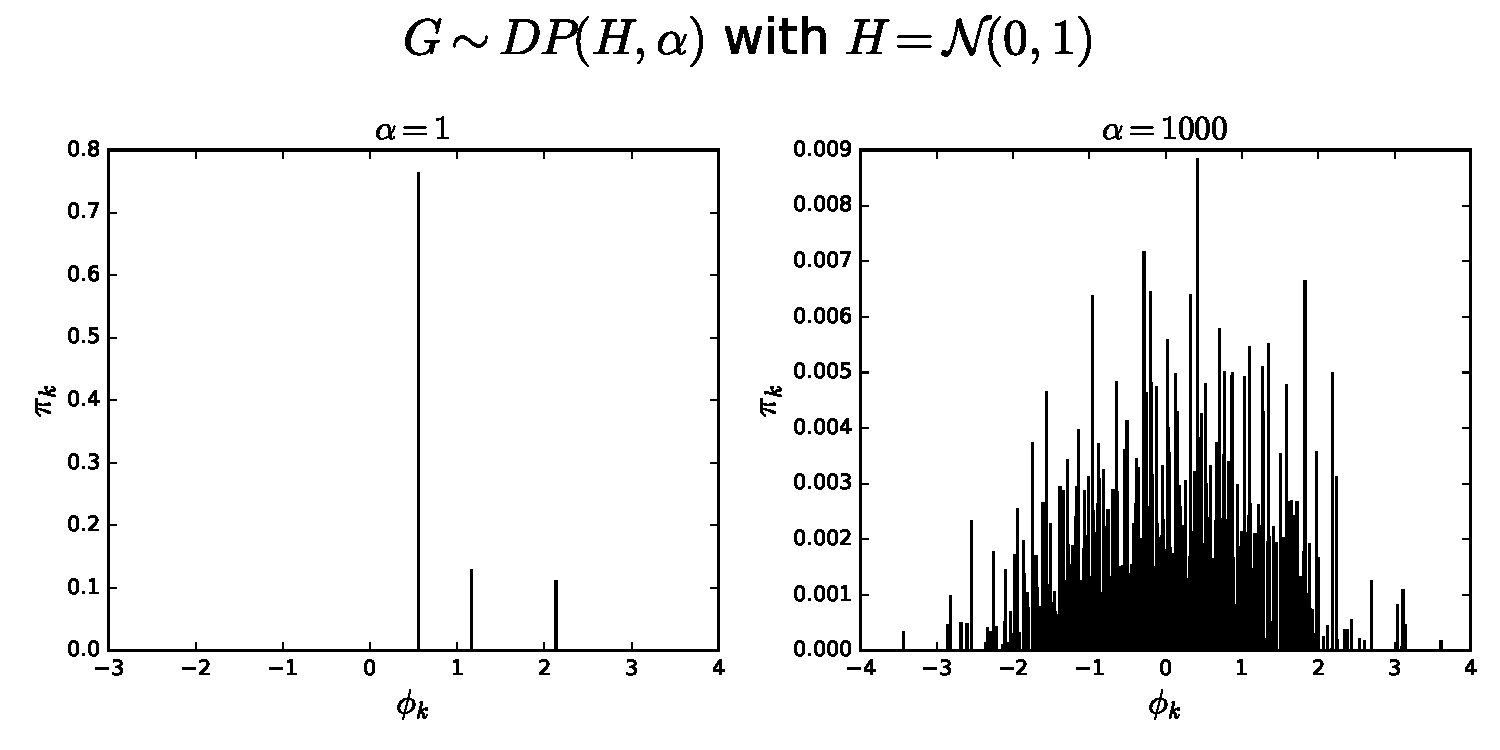
\includegraphics[width=1.0\textwidth]{03-machine-learning/figures/dp_samples_stick.pdf}
\par\end{centering}
\caption{\label{fig:g-from-dp-stick}Two samples of $G$ (up to a finite number of discrete points) generated by a Dirichlet Process with $\alpha=1$ (left) and $\alpha=1000$ (right) and a base distribution $\mathcal{N}(0, 1)$. We see that $\alpha$ affects how smooth the resulting discretisation of $H$ is in $G$.}
\end{figure}

Figure~\ref{fig:g-from-dp-stick} shows two examples of $G$ drawn from a DP with a Gaussian base distribution, $H=\mathcal{N}(0, 1)$ and varying values for $\alpha$. As noted earlier, a key property of the DP is that $G$ is a discrete distribution despite $H$ being continuous. The level of discretisation of $H$ is controlled by $\alpha$, with small $\alpha$ resulting in fewer discrete points with larger probabilities in $G$ and large $\alpha$ causing $G$ to have more discrete points. Since $\boldsymbol{\pi}$ is discrete and sums to 1, sampling from $G$ will generate repeated values. This illustrates the usefulness of the DP, in particular for clustering by setting the DP as a prior over the distribution of the mixture components. 

We also show in Figure~\ref{fig:g-from-dp} how the generative process in eq. (\ref{eq:background-infinite-mixture-dp}) works. First we sample a distribution $G$ from the DP parameterised by $\alpha$ and a base distribution $H$. In the example of Figure~\ref{fig:g-from-dp}A, the base is set to $\mathcal{N}(0, 1)$ and $G$ contains two unique discrete values, denoted by the red and green crosses, each of which is also a cluster component mean $\mu_k$. Every $n$-th data point is associated with a $\mu_k$, and each $\mu_k$ generates the data for its cluster by sampling for values from $\mathcal{N}(\mu_k, sigma^2)$. 
\begin{figure}
\noindent \begin{centering}
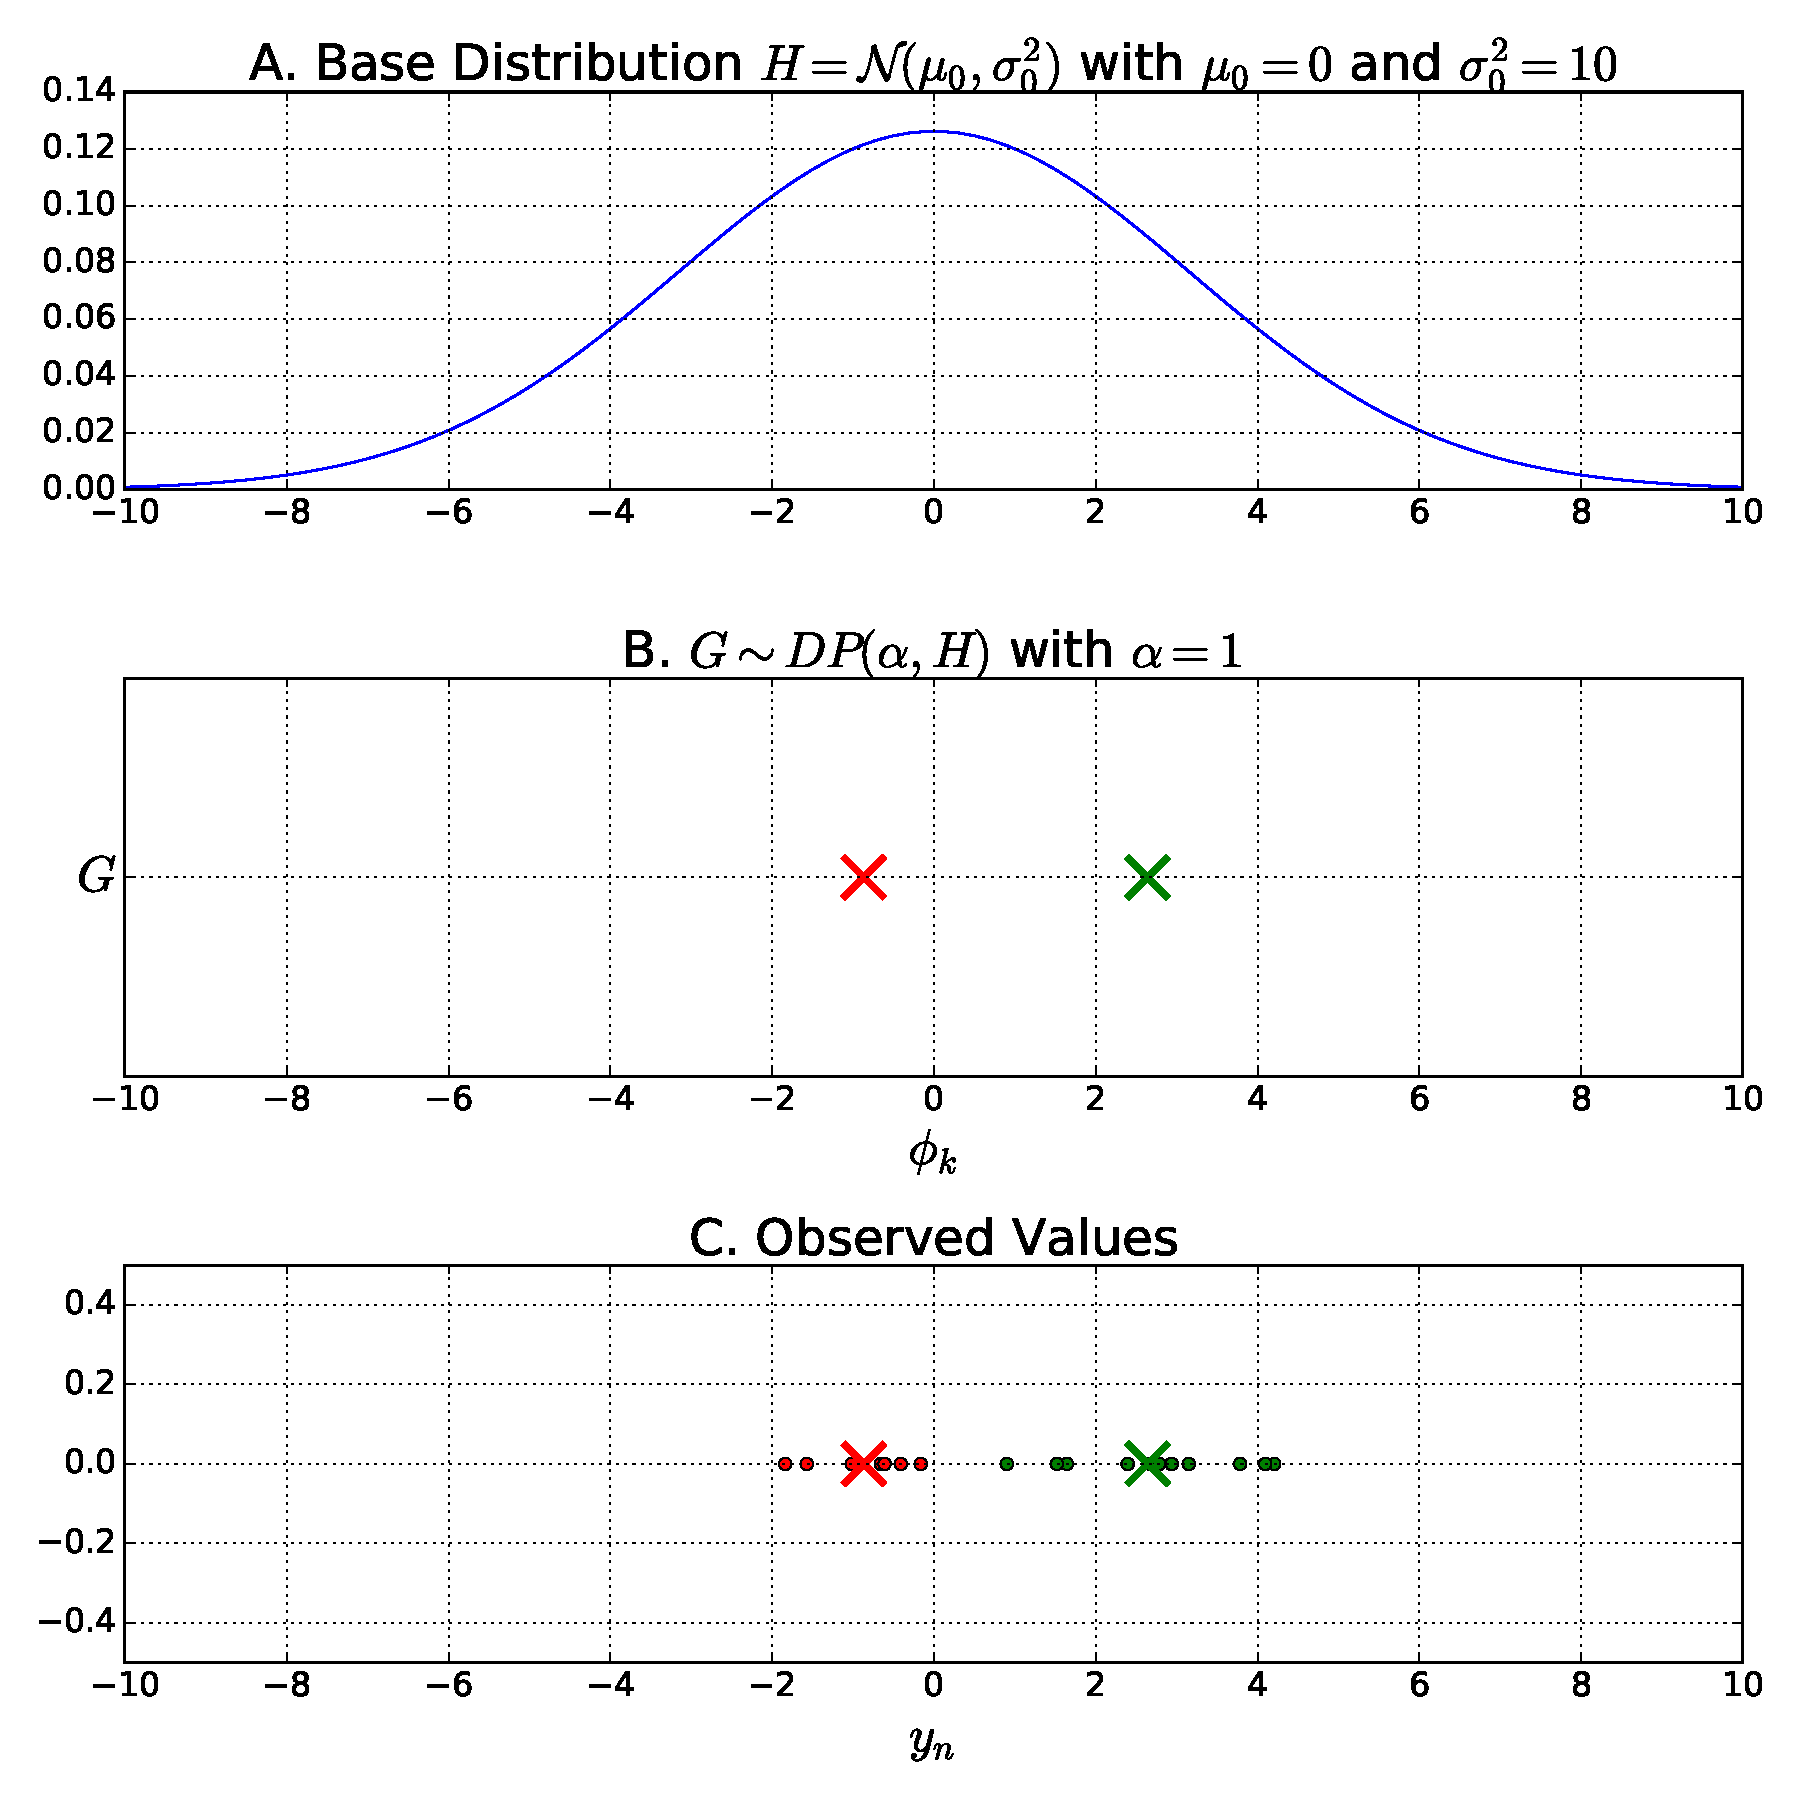
\includegraphics[width=0.6\textwidth]{03-machine-learning/figures/dp_samples.pdf}
\par\end{centering}
\caption{\label{fig:g-from-dp}An illustration of the generative process for the DP mixture model in eq. (\ref{eq:background-infinite-mixture-dp}). First, we require a base distribution to sample for discrete values, shown in \textbf{(A)}. Given $H$ and some concentration parameter $\alpha$, we generate a discrete distribution $G$. In \textbf{(B)}, we see that $G$ contains two unique discrete values sampled from $H$, represented by the red and green crosses. Each discrete value in G $\phi_k$ is also a cluster mean $\mu_k$. \textbf{(C)} The noisy observed values is generated by sampling for $\mu_k$ from $G$, and sampling for $y_n$ conditioned on the $\mu_k$.}
\end{figure}

\subsection{Collapsed Gibbs Sampling for an Infinite Mixture Model}

Having defined the generative process for an infinite mixture model, we are now interested in performing inference on the model parameters. In particular for Gibbs sampling, we require the probability of the current $n$-th data point that is being sampled to be in a cluster ($P(z_{nk}=1$), conditioned on the assignments of other data points ($\boldsymbol{Z}^{-}$). We show how we derive this by modifying the original collapsed Gibbs sampler as the number of components $K$ goes to infinity. Assuming a symmetric prior on the Dirichlet hyperparameter, $\alpha_k=\frac{\alpha}{K}$, then the conditional probability on the assignment of peak $n$ to cluster $k$ from eq. (\ref{eq:background-integrated-pi}) becomes:
\begin{equation}
P(z_{nk}=1 \vert \boldsymbol{Z}^{-}, \boldsymbol{\alpha}) = \frac{c_k^{-n} + \frac{\alpha}{K}}{\alpha+N-1}
\label{eq:background-integrated-pi-symmetric}
\end{equation}
Taking the limit of eq. (\ref{eq:background-integrated-pi-symmetric}) as $K$ goes to infinity results in the following conditional probability for $z_{nk}=1$:
\begin{equation}
P(z_{nk}=1 \vert \boldsymbol{Z}^{-}, \boldsymbol{\alpha}) = 
\begin{cases}
    \frac{c^{-n}_k}{\alpha+N-1}, & \text{for existing clusters} \\
    \frac{\alpha}{\alpha+N-1}, & \text{for a new cluster}
\end{cases}
\label{eq:background-crp}
\end{equation}
The conditional probability in eq. (\ref{eq:background-crp}) is also often formulated as the Chinese Restaurant Process (CRP) \cite{frigyik2010introduction}. In this process, an analogy is proposed based on a Chinese restaurant having an infinite number of tables. Tables correspond to clusters while customers correspond to the observed data points. The CRP is a random process that defines the probability of a customer to sit at a particular table, conditioned on the seating arrangements of other customers. For a non-empty table, this probability is proportional to $c_k$, the number of other customers seated at a table, while for an empty table, the probability is proportional to $\alpha$. Under exchangeablity, the joint posterior distribution in the CRP is invariant to the ordering of the items \cite{aldous1985exchangeability}. This means we can assume that the $n$-th data point is the last customer to arrive in the CRP, and the conditional probability for $P(z_{nk}=1)$ is thus proportional to eq. (\ref{eq:background-crp}). Coupled with a likelihood for a data point to be assigned to a table, we can use this to modify our conditional probability for Gibbs sampling, resulting in:
\begin{equation}
P(z_{nk}=1 \vert \boldsymbol{Z}^{-}, \boldsymbol{\alpha}) \propto 
\begin{cases}
    c^{-n}_k \cdot p(y_n \vert \boldsymbol{Z}^{-},  \boldsymbol{y}^{-}, \mu_0) \\
    \alpha \cdot p(y_n \vert \mu_0)
\end{cases}
\label{eq:background-infinite-mixture-model-sampling}
\end{equation}
The top term in eq. (\ref{eq:background-infinite-mixture-model-sampling}) corresponds to the probability of being assigned to non-empty (existing) clusters. As in the finite mixture model case, this prior probability is proportional to $c^{-n}_k$, the number of data points (peaks) currently assigned to cluster $k$ excluding the $n$-th peak that is being sampled, while the likelihood $p(y_n \vert \boldsymbol{Z}^{-},  \boldsymbol{y}^{-}, \mu_0)$ is defined in eq. (\ref{eq:background-tilde-mu-sigma-variance}) or equivalently in eq. (\ref{eq:background-tilde-mu-sigma-precision}) when precision is used. The bottom term in eq. (\ref{eq:background-infinite-mixture-model-sampling}) corresponds to the probability of creating a new cluster with the prior probability proportional to $\alpha$ and likelihood $p(y_n \vert \mu_0)$. In this particular case due to conjugacy, we can derive the likelihood $p(y_n \vert \mu_0)$ by marginalising over all empty components, resulting in:
\begin{equation}
\begin{aligned}
p(y_n \vert \mu_0) &= \int p(y_n \vert \mu_k) p(\mu_k \vert \mu_0) \enspace d_{\mu_k}
                               &= \mathcal{N}(y_n \vert \mu_0, \sigma^2 + \sigma_0^2)
\end{aligned}
\label{eq:background-new-table-likelihood}
\end{equation}
In other cases where it is not possible to derive the data likelihood analytically, we can approximate it by sampling from the prior instead \cite{Rasmussen2000}. This completes the necessary modification to our collapsed Gibbs sampler. The sampling process proceeds largely as before by removing the $n$-th peak from the model and performing the assignment of that peak to cluster $k$ using eq. (\ref{eq:background-infinite-mixture-model-sampling}). If an existing $k$ is selected, this is then the same as the finite mixture case. When a new $k$ is selected, we create a new cluster and assign the peak to that cluster. In this manner, the number of mixture components is not fixed in advance \textit{a priori}, but is instead determined based on the observed data and the choice of hyperparameter $\alpha$.

\section{Hierarchical Dirichlet Process Mixture Model Clustering\label{background-hdp-clustering}}

While the DP mixture model allows us to cluster related peaks together, the clustering process within each run is performed separately and independently of the others. However, in some cases it is useful to allow for clustering to be shared across runs. We call the clusters shared in this manner to be the \emph{global clusters}, as opposed to the \emph{local clusters} that are found in each file. In LC-MS data, global clusters can be assumed to correspond to compounds (e.g. metabolites or peptide fragments) that are present in all runs, while local clusters are the noisy realisation of such global clusters in each run. Often, the shared presence of global clusters can be assumed when we have multiple runs generated from the measurements of the same biological sample. In this case, the runs are called technical replicates. In other circumstances when the runs are generated through the measurements of different biological samples, shared compounds might also be found and can therefore be represented as global clusters.

Hierarchical Dirichlet Process (HDP) mixture model is an extension of the DP mixture model that allows for such global clusters to be defined and shared across multiple runs \cite{teh2005hierarchical,teh2012hierarchical}. Within each file, the observed data points are clustered into local clusters, which are assigned to the shared global clusters. In our application, the HDP mixture model is particularly useful for alignment as being able to generatively explain which peaks are generated by which global clusters is the same as being able to match these peaks across runs. This application is shown in Chapter~\ref{c:hdp} where we introduce a HDP mixture model to simultaneously group peaks within and across runs. From the model, the matching of peaks (alignment) is constructed from the marginal probabilities of peaks to be assigned into the same global cluster. 

To understand the HDP mixture model, first we need to define the hierarchical Dirichlet Process. Given a concentration parameter $\alpha_0$ and a base distribution $H$, let $G_0$ to be a distribution sampled from a $DP(\alpha_0, H)$. Then for each file $j=1,...J$, we can sample a file-specific distribution $G_j$ from another Dirichlet Process parameterised by $\alpha_j$, with $G_0$ as its base distribution. This file-specific DP is denoted as $DP(\alpha_j, G_0)$.
\begin{equation}
\begin{aligned}
G_0 \vert \alpha_0, H &\sim DP(\alpha_0, H) \\
G_j \vert \alpha_j, G_0 &\sim DP(\alpha_j, G_0)
\end{aligned}
\label{eq:background-hdp-process}
\end{equation}
As a property of the DP, $G_0$ is a discrete distribution with probabilities that sums to 1 (regardless of whether $H$ is continuous or discrete). This means $G_0$ has a support over the discrete values ${\phi_1, \phi_2, ... }$ that have been drawn from its base distribution $H$. We use $G_0$ to represent the prior distribution over the global components. Each $G_j$ is a prior distribution over the file-specific local components, and since $G_j$ is drawn from a DP with $G_0$ as its base distribution, each $G_j$ is discrete and has a support over the same discrete values as $G_0$. This is where the sharing property of the HDP comes about. The sets of discrete values in $G_0$, which represent the prior values on the global components, are inherited (copied) to the discrete values in $G_j$ that represent the prior values on the local components.

To define a HDP mixture model, we complete the hierarchical prior defined in eq. (\ref{eq:background-hdp-process}) with a data-generating distribution. Let $j=1,...,J$ indexes over the input files (LC-MS runs), while the $n$ indexes over the number of peaks in a particular $j$-th file. Assuming that the noise on the observed RT values is Gaussian-distributed, together with eq. (\ref{eq:background-hdp-process}), we obtain the following generative model for a HDP mixture model:
\begin{equation}
\begin{aligned}
\mu_j \vert G_j            &\sim G_j \\
y_n \vert \mu_k           &\sim \mathcal{N}(y \vert \mu_k, \sigma^2)
\end{aligned}
\label{eq:background-infinite-mixture-hdp}
\end{equation}

This generative process from the HDP mixture model in eq. (\ref{eq:background-infinite-mixture-hdp}) is also illustrated in Figure~\ref{fig:g-from-hdp}. Note the key difference between HDP mixture (Figure~\ref{fig:g-from-hdp}) and the DP mixture (Figure~\ref{fig:g-from-dp}). The addition of another level of hierarchy to the HDP mixture model, where the discrete values in $G_{j}$ for each file $j$ is drawn from anothe DP having $G_{0}$ as its base, makes it possible for clustering parameters to be shared across files. 

Figure~\ref{fig:g-from-hdp} also reveals that within a file-specific $G_j$, each discrete value is copied exactly from the base distribution $G_0$. This may not be what we want. Particularly in our application, the top-level $G_0$ is the prior distribution over global compounds (metabolites/peptides), while the file-specific $G_j$ is the prior distribution over the realisation of those compounds within a file. It is reasonable to expect the discrete values in $G_j$ to vary from $G_0$ due to the addition of random noise that represents RT drift. The addition of noise in this manner results in the `HDP with random effects' model \cite{kim2006hierarchical}, and indeed our proposed HDP mixture model in Chapter~\ref{c:hdp} resembles this but includes the addition of LC-MS-specific features. Gibbs sampling has been used for inference in the HDP mixture model \cite{teh2005hierarchical}, and in Chapter~\ref{c:hdp}, we also describe the construction of a Gibbs sampling for this purpose.

\begin{figure}
\noindent \begin{centering}
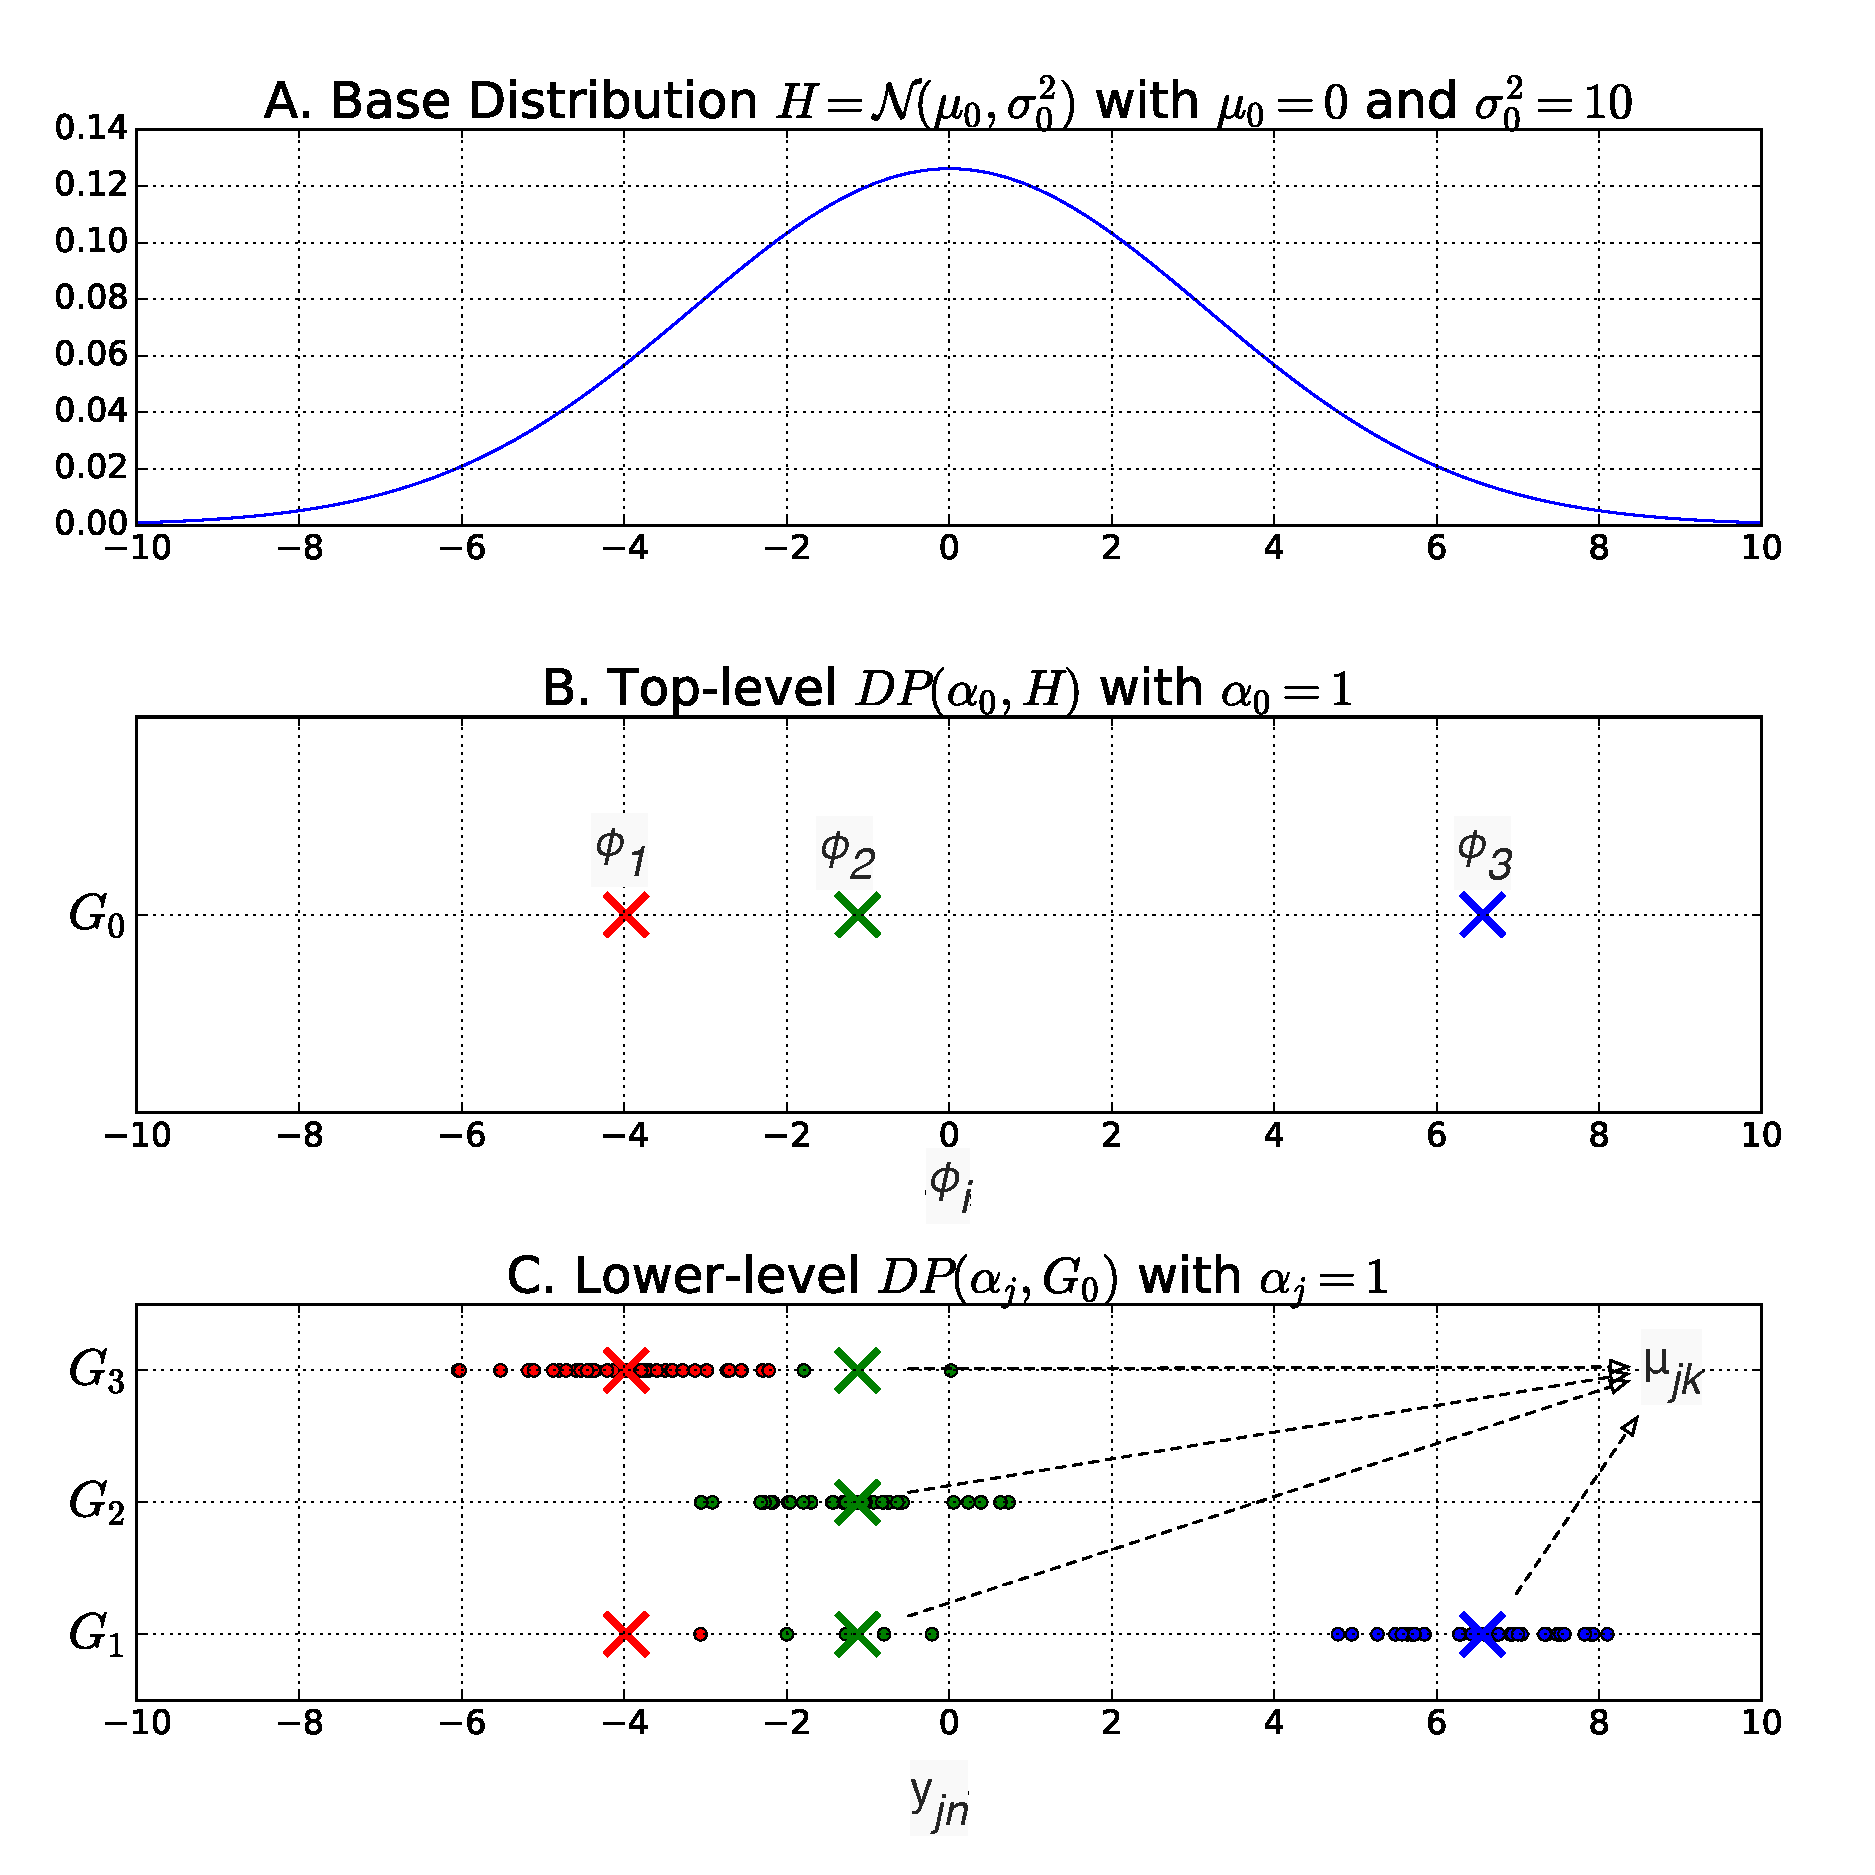
\includegraphics[width=0.6\textwidth]{03-machine-learning/figures/hdp_samples.pdf}
\par\end{centering}
\caption{\label{fig:g-from-hdp}An illustration of the generative process for the HDP mixture model in eq. (\ref{eq:background-infinite-mixture-hdp}). Similar to the DP mixture, we have a base distribution shown in \textbf{(A)}. Given $H$ and some concentration parameter $\alpha$, we generate a global distribution $G_0$. In \textbf{(B)}, we see that $G_0$ contains three unique discrete values. We then generate a file-specific distribution $G_j$ by sampling from a DP with $G_0$ as the base distribution. As a consequence, $G_j$ contains only discrete values copied from $G_0$. In \textbf{(C)}, the noisy observed values within each file is generated by sampling for $\mu_k$ from $G_j$, and sampling for $y_n$ conditioned on the $\mu_k$.}
\end{figure}

\section{Latent Dirichet Allocation\label{background-lda}}

TO FINISH

Latent Dirichlet Allocation (LDA), proposed in \cite{Blei2003}, is a probabilistic topic model widely used for unsupervised topic discovery. In the standard LDA model applied to text mining, documents comprise of some topics, each of which may produce the observed words in that document. Given a corpus of documents, the goal of inference in LDA is to approximate the posterior distributions of documents to topics and words to topics. Any other topic models??

For the purpose of substructure discovery in MS2 data, a topic -- explained as the set of recurring words shared in many documents -- can be seen as corresponding to a substructure shared by many metabolites. Each topic then produces the observed MS2 fragment/loss words in an MS1 document. We assume the bag-of-word word model, where within each MS1 document, the observed MS2 fragment/loss word features are exchangeable. i.e. their ordering do not matter, only their observed counts matter. The input to LDA is therefore a matrix of the counts of occurences of MS2 word for each MS1 document. This can produced by concatenating the count matrices of the fragment words and the loss words produced in section \ref{sec:Feature-Extraction} row-wise, e.g. if there are $N_{f}$ unique fragment words and $N_{l}$ unique loss words, both of which are shared across $D$ MS1 peaks, the input matrix to LDA is a $D$-by-$(N_{f}+N_{l})$ matrix. Entries in the matrix are the observed counts of words in the document, so they are the discretised intensity values of the fragment and loss words for each MS1 peak -- produced according to Section \ref{sec:Feature-Extraction}. We restrict the input to the standard LDA to take into account only the fragment and loss words because the counts of both fragment and loss words are derived from the normalised intensity values of the MS2 peaks.

The standard LDA model -- as applied to substructure discovery -- is now briefly described here. Given $K$ predefined topics (indexed by $k=1,...,K$) corresponding to metabolite substructures, the observation of the $n$-th MS2 fragment/loss word in the $d$-th document (MS1 peak) can be described by the following generative process.
\begin{equation}
w_{dn}|\boldsymbol{\phi}_{z_{dn}}\sim Multinomial(\boldsymbol{\phi}_{z_{dn}})
\end{equation}
\begin{equation}
z_{dn}|\boldsymbol{\theta}_{d}\sim Multinomial(\boldsymbol{\theta}_{d})
\end{equation}
\begin{equation}
\boldsymbol{\theta}_{d}|\alpha\sim Dirichlet(\alpha)
\end{equation}
\begin{equation}
\boldsymbol{\phi}_{k}|\beta\sim Dirichlet(\beta)
\end{equation}
In other words: observation on the $n$-th MS2 word in the $d$-th MS1 peak ($w_{dn}$) is conditioned on the assignment of word $w_{dn}$ to some known $k$-th multinomial distribution (corresponding to a substructure). This assignment is denoted by the indicator variable $z_{dn}$, so $z_{dn}=k$ if $w_{dn}$ is assigned to a $k$-th multinomial. The $k$-th multinomial distribution that an MS2 word is assigned to is characterised by the parameter vector $\boldsymbol{\phi}_{z_{dn}}$. However, $\boldsymbol{\phi}_{z_{dn}}$ is itself drawn from a prior Dirichlet distribution having a symmetric parameter $\beta$. The probability of seeing certain substructures (topics) for each $d$-th MS1 peak is then drawn from a multinomial distribution with a parameter vector $\boldsymbol{\theta}_{d}$. This parameter vector $\boldsymbol{\theta}_{d}$ is in turn drawn from a prior Dirichlet distribution having a symmetric parameter $\alpha$. Figure \ref{fig-platediagram} is the plate diagram of the standard LDA model, which shows the conditional dependencies between the random variables in the model.

\section{Conclusion}

...